\documentclass[a4page,11pt]{article}
\usepackage[utf8]{inputenc}
\usepackage{amsmath,amssymb,amsfonts}
\usepackage{graphicx}

\renewcommand{\vec}[1]{\mathbf{#1}}%
\newcommand{\mat}[1]{\mathbf{#1}}%
\newcommand{\est}[1]{\hat{#1}}%
\newcommand{\set}[1]{\mathcal{#1}}%
\newcommand{\iter}[1]{^{(#1)}}%
\newcommand{\spc}[1]{\mathbb{#1}}%
\newcommand{\expe}[2]{\mathbb{E}_{#1}\left[#2\right]}%
\newcommand{\prob}[1]{\mathrm{Pr}\left\{#1\right\}}%
\newcommand{\ind}[1]{\mathbf{1}\left(#1\right)}%
\newcommand{\setdef}[1]{\left\{#1\right\}}%
\newcommand{\tuple}[1]{\left(#1\right)}%
\newcommand{\norm}[1]{\left\|#1\right\|}%

\def\gauss{\mathcal{N}}%
\def\ber{\mathrm{Ber}}%
\def\uni{\mathrm{Uni}}%
\def\obs{\mathcal{O}}%
\def\opt{^{*}}%
\def\tra{^T}%
\def\inv{^{-1}}%
\def\pinv{^{\dagger}}%
\def\reals{\mathbb{R}}%

\author{R. Grompone and I. Ramírez and G. Randall}
\title{Mamatrote}

\begin{document}

\begin{abstract}
This work describes a general method for the detection of different types of structures in a set of elements that belong to a certain ambient space. The general idea is that such structures express themselves as unusual concentrations of subsets of such elements around these structures, as opposed to being randomly scattered throughout the space. 
\end{abstract}

\section{Preliminaries}


\paragraph{Notation}

\begin{itemize}
\item Dimensions are lower capital letters such as $m,n,p$. Random variables are capital letters such as $X,Y,Z$. 
\item Vectors are lower case bold, e.g., $\vec{x}$. 
\item Matrices are upper-case bold as in $\mat{A}$. 
\item Spaces are in double bold, such as $\mathbb{R},\mathbb{C},\mathbb{X}$.
\item Sets are in calligraphic, such as $\set{O}$; their cardinality is written as $|\set{O}|$
\item The probability of a given event $\omega$ is $\prob{\omega}$. 
\item $\expe{X}{f(X)}$ is the expectation of the function $f(X)$ w.r.t. the distribution of $X$.
\item The indicator function is denoted as $\ind{A=1}$
\item For a vector $\vec{x}$, the $i$-th element is denoted as $x[i]$
\item For elements in a set, the $j$-th element of a set is denoted as $x_j$
\item Combining both definitions above, the $i$-th element of the $j$-th vector in a set of vectors is denoted by $\vec{x}_j[i]$.
\end{itemize}

\paragraph{Conventions}
Letters such as $i,j,k,l,r$ are reserved for indexes. The letter $t$ indicates  iteration number. Letters such as $m,n,p$ are for dimensions. $a,b,c$ are usually constants. $d$ is used for distances,  $e$ for errors, $f,g,h$ for functions. $u,v,w,x,y,z$ usually denote realizations of correponding random variables $U,V,W,X,Y,Z$. The letters $x,y,z$ can also denote 2D/3D spatial coordinates.
Greek letters $\alpha,\beta,\gamma,\tau$ are usually system hyperparameters (such as a threshold $\tau$), whereas $\mu,\theta,\sigma$ are commonly used for PMF/PDF parameters.

\section{Problem Setting}

The task is to detect meaningful structures hidden among the set of observed elements. We begin by restricting such structures to a parametric family $\space{Q}$. We begin by considering $\space{Q}$ to be the set of affine subspaces of a given dimension $m$ on an ambient space of dimension $n$.

We represent affine subspaces as a triplet $(\vec{u},\mat{V},\mat{W})$ where $\vec{u}$ is the distance of the set to the origin, $\mat{V}$ is a matrix whose columns generate the affine space, and $\mat{U}$ is the orthogonal complement of $\mat{V}$.

A generic point in the ambient space is represented by $\vec{x} \in \reals^n$. The set of observed data points is $$\set{X} = \setdef{ \vec{x}_1,\vec{x}_2,\ldots,\vec{x}_N}.$$. Alternatively, we might represent this dataset as a matrix $\mat{X} \in \reals^{n{\times}N}$ whose columns are the data points.

The notion of \emph{concentration} arond a model $q$ implies a metric and a distance. We denote the distance from a point $\vec{x}$ to any model $q$ is $d(o,m) \in \reals^+$ as $d(\vec{x},q)$. For affine sets, the distance is defined as the norm of the distance between $\vec{x}$ and its projection $\Pi_q(\vec{x})$ onto $q$. 

Any given point is considered to belong to some model $q$ or either the \emph{background}. Thus, we need to provide a model for the background as well (this would be the \emph{null hypothesis} in classical statistics). The main contribution of this work is to consider \emph{local} background models that are defined relative to a region around a given candidate model $q$. The reason for this will become clear later.


\section{General detection framework}

The general detection pipeline involves the following steps:

\begin{itemize}
\item Define the model family and the background model
\item Find a set of candidate models $\set{Q}$
\item For each model $q \in \set{Q}$, define \emph{local background model} $\hat{q}$ representing the abscence of evidence for that model; this is in contrast to other works, which consider a global background model, such as a uniform distribution over a compact subset of the ambient space.
\item keep those models which pass the \emph{significance test} in a set $\set{S}^+$
\item Generate a set of \emph{refined models}, $\set{S}\opt$, by  removing those models in $\set{S}$ that are \emph{redundant} w.r.t. some criterion. 
\end{itemize}

The above pipeline is quite standard in many detection frameworks. The novel aspect of this work lies in performing a \emph{significance test} w.r.t. a \emph{local} background model. This in turn calls for novel ways of defining such tests. This is where most of our work will be devoted to. 

On the other hand, finding a proper set of candidate models is a very difficult problem. Clearly, the family $\spc{Q}$ is infinite and generally uncountable. Even if we restrict ourselves only to those models that can be determined by subsets of objects (e.g., all line segments defined by all pairs of points in $\set{X}$), the number of candidates can be huge.
Thus, for now and most of this work, we will assume $\set{Q}$ to be given to us.


\subsection{Background model}


\begin{figure}
\centering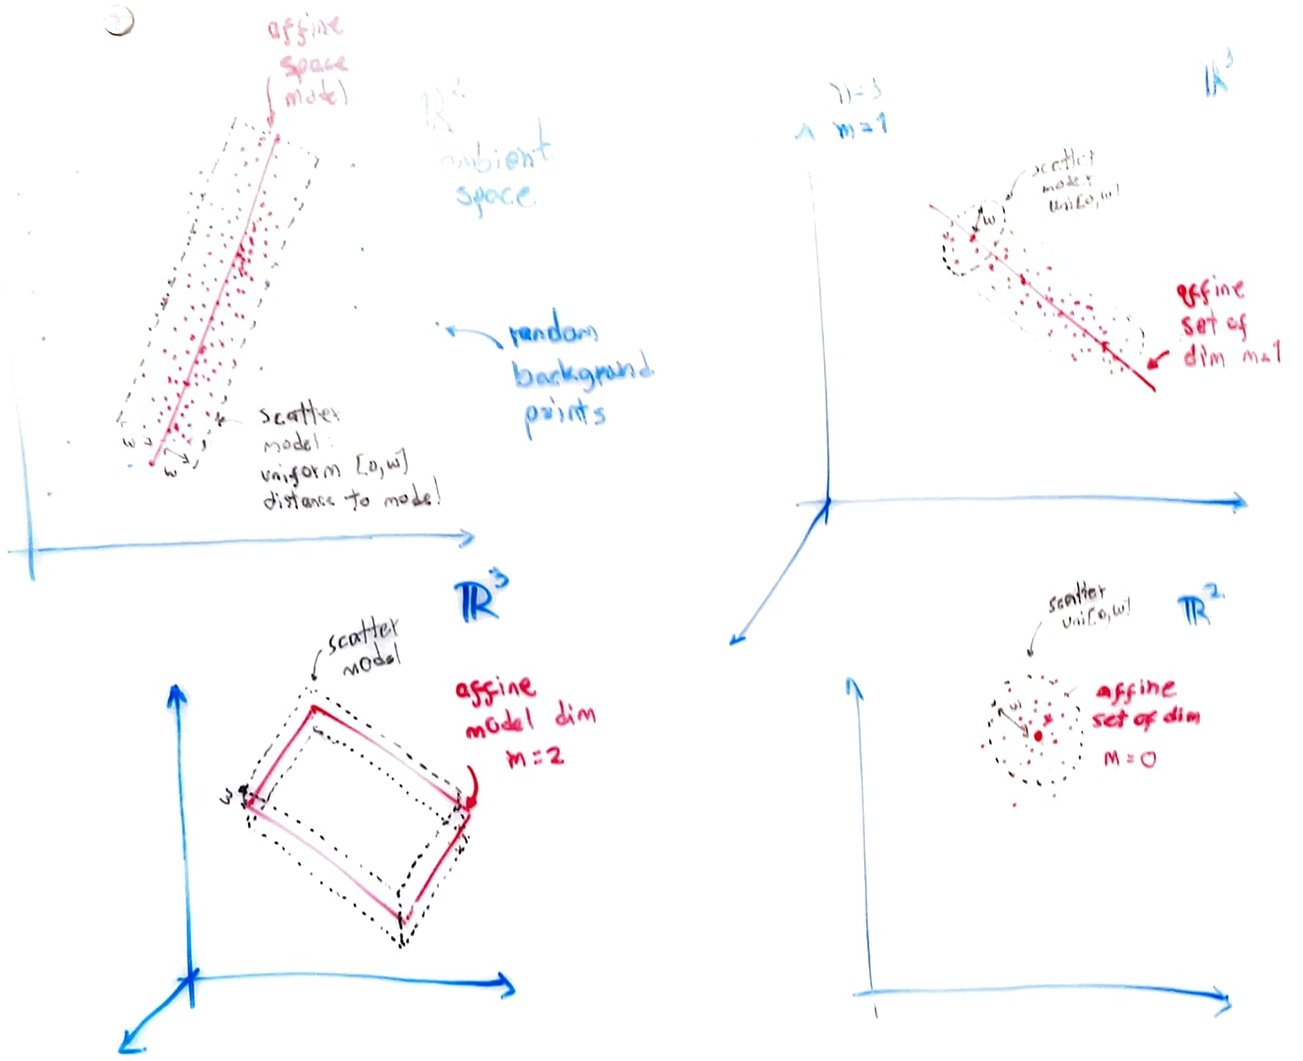
\includegraphics[width=0.9\textwidth]{examples}
\caption{\label{fig:examples}Examples of some affine sets (in red), ambient spaces, and local background (scatter) models (in black). Notice that single points are considered zero-dimensional affine sets.}
\end{figure}

\begin{figure}
\centering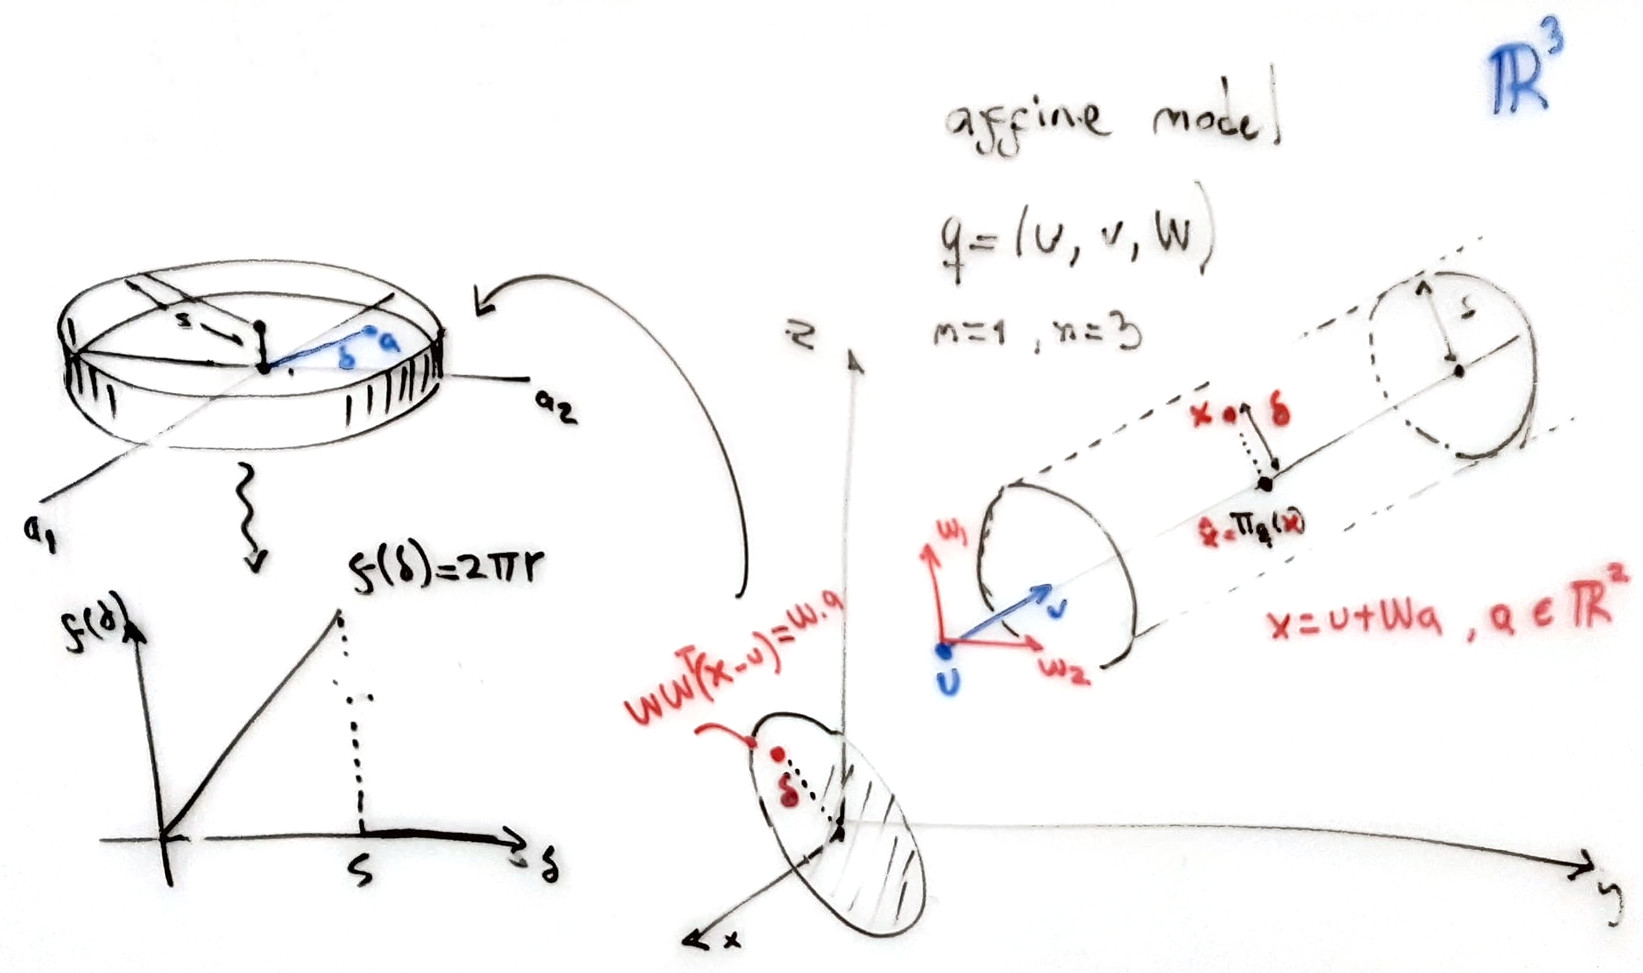
\includegraphics[width=0.7\textwidth]{intuition}
\caption{\label{fig:intuition}Some intuition behind the background model. The example $q$ here is a one-dimensional affine set (a line) on a 3D Euclidean space. In this setting we have $\vec{u} \in \reals^{3}$, $\mat{V} \in \reals^{3{\times}1}$ and $\mat{W} \in \reals^{2{\times}3}$. Given points of the form $\vec{x}=\vec{u}+\vec{W}\vec{a}+\vec{V}\vec{b}$, the density of $\vec{a} \in \reals^2$ is uniform on the 2D disk or radius $s$, which in turn generates a uniform distribution on the distance of points in the disk to the origin whose  density is linear function truncated at $s$, in this case it is simply $f(\delta)=2\delta/s^2$; in general, $f(\delta) \propto \delta^{n-m-1}$.}
\end{figure}


For an affine model of dimension $m$ on ambient space $n$, we consider points whose distance to $q$ is no larger than a given scatter parameter $s$. Formally speaking, such points belong to  the direct product of a sphere of dimension $n-m$ and the affine subsspace $q$; this is the local background model $\hat{q} = \setdef{a+b: a \in q, b \in \reals^{n-m}, \|b\|_2 \leq s}$. 

We further assume that background points are distributed uniformly in $\hat{q}$. Although this does not define a proper distribution, the distribution of the \emph{distance} to such points to $q$ is well defined. Indeed, any point  $\vec{x} \in \hat{q}$ can be written as $\vec{x} = \vec{u} + \vec{W}\vec{a} + \vec{b}\vec{V}$ with $\|\vec{a}\| \leq s$. Now, the distance of $\vec{x}$ to $q$ is given by 

$$\norm{\mat{W}\tra(\vec{x}-\vec{u})}_2=\norm{\mat{W}\tra(\mat{W}\vec{a}+\mat{V}\vec{b})}=\norm{\vec{a}}_2,$$

and $\vec{a}$ is supported on the closed ball in $\reals^{n-m}$, $\set{B}^{n-m}_s=\setdef{\vec{a}: \|\vec{a}\|_2 \leq s}$. Now, in turn, this uniform distribution on the sphere defines a distribution on the \emph{distance} $\delta$ of a point $\vec{x}$ in $\hat{q}$ to $q$. If we denote by $S^{n-m}_\delta$ the volume of the ball $\set{B}^{n-m}_\delta$, then the induced density is

$$f(\delta \leq z) = \frac{\set{B}^{n-m}_z}{\set{B}^{n-m}_s},$$

which, up to a constant is simply a truncated power law: 

$$\prob{\delta \leq z} = 
\left\{
\begin{array}{cc}
\kappa\delta^{n-m} & \mathrm{if}\;\delta \leq s \\
1 &\mathrm{otherwise} \\
\end{array}
\right.
$$
Figure~\ref{fig:intuition} on this.


\subsection{Significance test}

\begin{figure}
\centering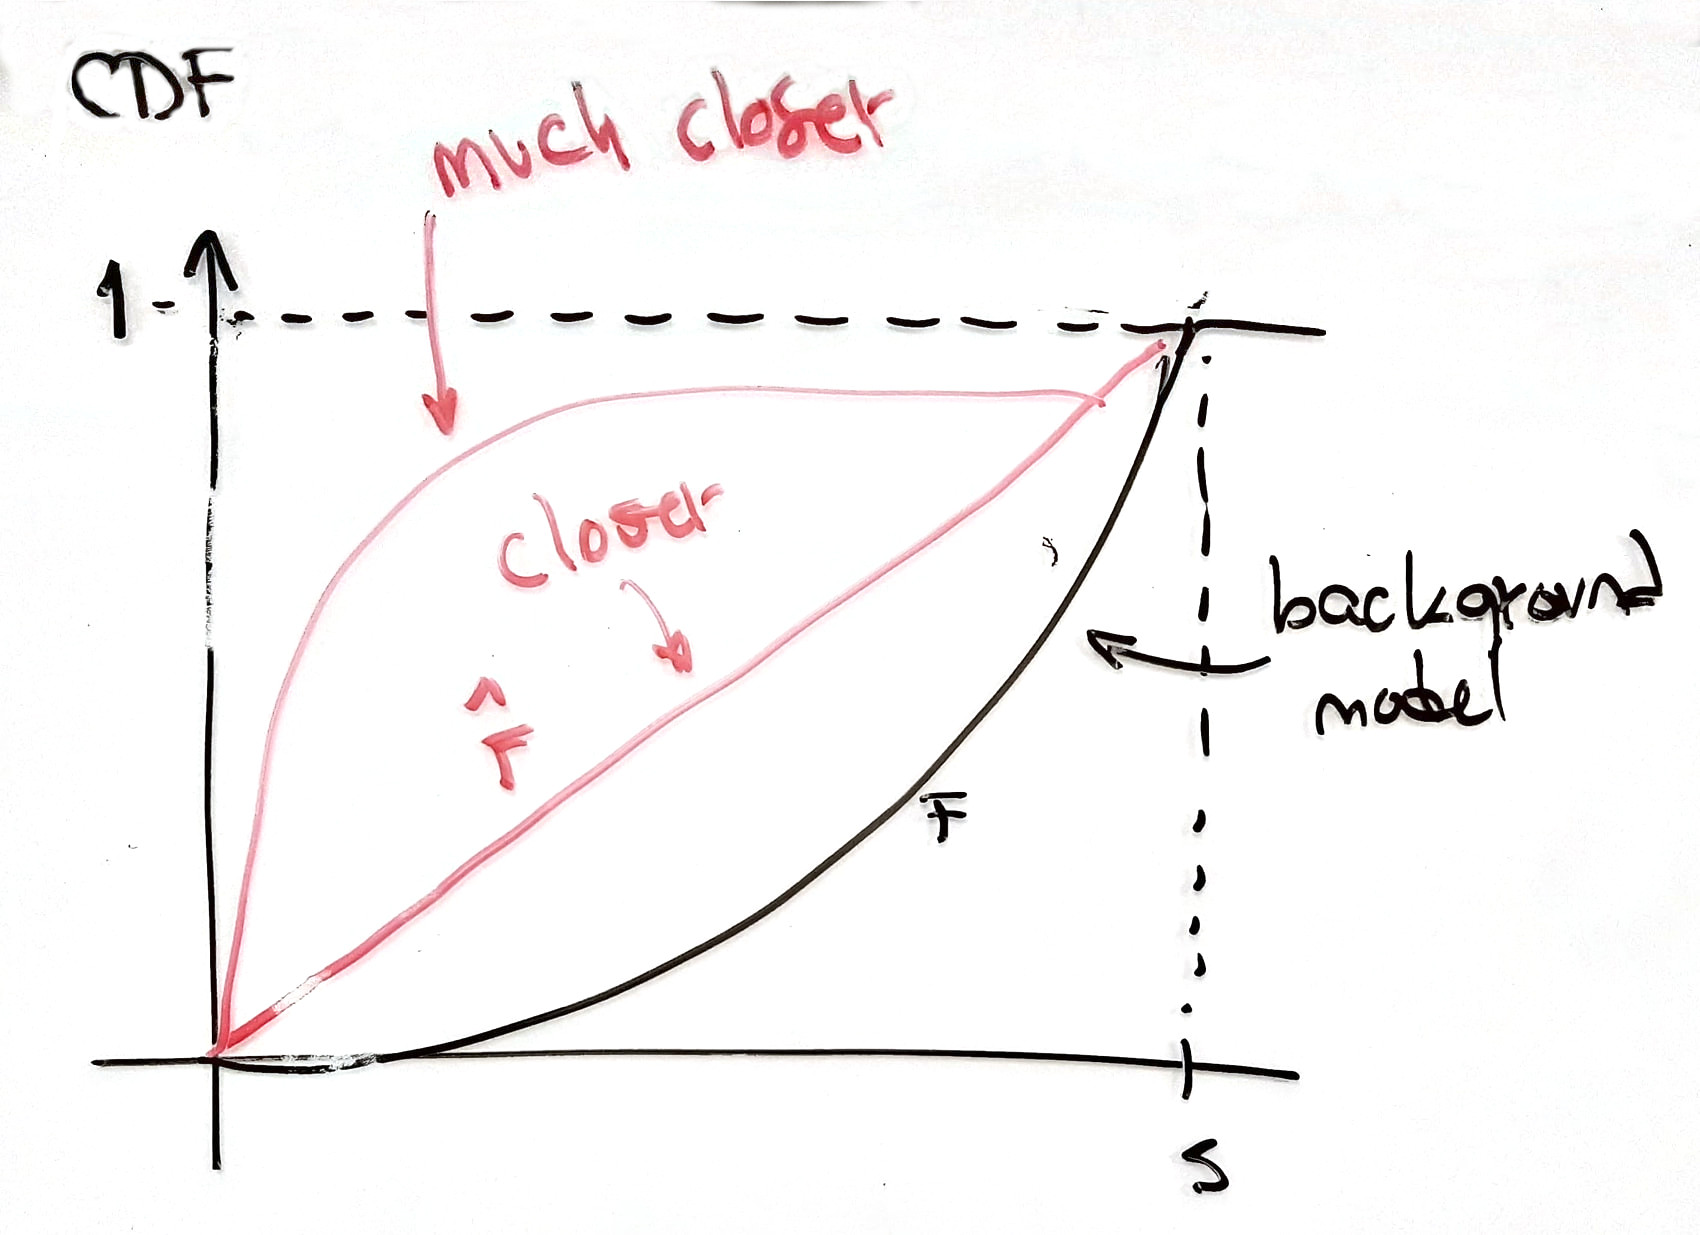
\includegraphics[width=0.5\textwidth]{significance}
\caption{\label{fig:significance} In black we see the background CDF for the distance $\delta$ for the case where $n-m=2$ (a 2D disk) and a couple of imagined empirical CDFs which would indicate that the concentration of points near the model $q$ is unusually high.}
\end{figure}


A given model $q$ will be considered significant if the points in $\hat{q}$ are unusually close to $q$ to be uniformly distributed. We can analyze this in terms of the empirical vs. expected  distributions of the distances $\delta$. The expected distribution is the one given by the background model, that is, $F(\delta) = \kappa \delta^{n-m}$. The empirical distribution is given by:

$$\hat{F}(\delta)=\frac{\sum_{\vec{x} \in \hat{q}} \ind{d(\vec{x},q) \leq \delta}}{\sum_{\vec{x} \in \hat{q}}1} $$

If the points are \emph{closer} to what one would expect, then the empirical CDF $\hat{F}(\delta)$  should be larger than the background CDF $F(\delta)$ for small $\delta$, and smaller for larger $\delta$. Figure~\ref{fig:significance} depicts this scenario.

Ideally, we would like to condense the above criterion in terms of a $p$-value, that is, of the probability that the discrepancy between the observed and background distributions differ in some way, and determine a significance threshold, e.g., to declare a detection if $p < 0.05$.

A standard method for such task is the Kolmogorov-Smirnov test. This test is defined in terms of the maximum absolute pointwise difference between $F$ and $\hat{F}$. Although this does not distinguish between negative or positive differences, and closer or farther values, it still serves to some extent and is a well established procedure, and thus constitutes our first approach to the problem.



\subsection{Analysis scale}

A critical parameter of the above procedure is the assumed maximum distance $s$ of points to a model $q$; we also call this parameter the \emph{scatter scale} or \emph{analysis scale}, as it is clearly related to the scale of the objects we want to recognize. This is a very sensitive parameter: different scales will often yield different results. Moreover, for sufficiently large $s$, given that data points are bounded, a detection will always be produced for any candidate object $q$! Thus, conjuring a method for setting this scale parameter automatically is an important aspect of our work. This is still work in progress. Meanwhile, we will continue with $s$ assumed to be known.

\subsection{Multiple tests}

In general, the set of candidate models $\set{Q}$ will contain several elements. Therefore, in order to reduce the number of false detections (NFA for abbreviation)  we need take this multiplicity into account. The standard approach is to use a Bonferroni correction, that is, to divide the detection threshold by the number of elements in $\set{Q}$.

\section{Technical details}

Here we describe two things: first, the detection algorithm; second, the  simmulations.


\subsection{Detection algorithm}

\paragraph{Inputs:} 
\begin{enumerate}
\item Dataset $\set{X}$ consisting of $N$ samples of dimension $n$
\item Set of candidate models $\set{Q}$ given as triplets $(\vec{u},\vec{V},\vec{W})$ so that points in the affine set are generated as $\vec{u} + \mat{V}\vec{b}$ and $\vec{W}$ is the orthogonal complement of $\mat{V}$.
\item Analysis scale $s$
\item Significance level $\alpha$
\end{enumerate}

\paragraph{Algorithm: for each candidate model $q$ in $\set{Q}$ (the number of elements in $\set{Q}$ is $N_T$}
\begin{enumerate}
\item Select all points in $\set{X}$ whose distance is less than or equal than $s$, $\set{X}' = \setdef{\vec{x} \in \set{X}: d(\vec{x},q) \leq s)}$.
\item Compute empirical distribution of distances in $\set{X}'$
\item Compute the Kolmogorov-Smirnov score using the variant that only considers the largest \emph{positive} difference beteween the empirical and background distribution
\item Declare a detection if the KS score is below $\alpha/N_T$
\end{enumerate}

\subsection{Simmulation}

\paragraph{Inputs:} 
\begin{enumerate}
\item Total number of points $N$
\item Proportion of points that go to all the models, $\rho$
\item Number of ground truth models, $M$
\item Ambient space dimension $n$
\item Affine space dimension $m < n$
\item Distribution $g()$ used to displace model points from their exact position (e.g., Laplacian)
\item Scatter ratio $\sigma$: scale of displacement distribution
\end{enumerate}

\paragraph{Algorithm:}
\begin{enumerate}
\item Draw $(1-\rho)N$ background points so that their coordinates are uniformly distributed between $0$ and $R$
\item Repeat $M$ times:
  \begin{enumerate}
  \item Draw $m+1$ points $\setdef{\vec{y}_0,\vec{y}_1,\ldots,\vec{y}_m}$ in the same way as the background
  \item Set $\vec{u} = \vec{y}_0$
  \item Set $\vec{y}'_i = \vec{y}_i - \vec{u}$
  \item Construct an orthogonal basis $\mat{V}$ for the affine set using 
$\setdef{\vec{y}'_1,\ldots,\vec{y}'_m}$
  \item Construct $\mat{W}$, a basis for the orthogonal complement of $\mat{V}$
  \item Add $q=(\vec{u},\mat{V},\mat{W})$ to the set of ground truth models
  \item Draw $K=\rho/M$ random $\reals^m$ points $\setdef{\vec{b}_1,\ldots,\vec{b}_{K}}$  so that $b_i \sim \mathrm{Uni}(0,R)$
  \item Draw $K=\rho/M$ random $\reals^{n-m}$ points $\setdef{\vec{a}_1,\ldots,\vec{a}_{K}}$  so that $\|a_i\|_2 \sim g(\delta)$ and the direction of $\vec{a}$ is uniformly distributed. This is easy to approximate by first sampling from a Gaussian distribution and then rescaling the points to norm $\delta$ where $\delta$ follows the desired distribution
  \item Construct model points $\vec{x}_i = \vec{u} + \mat{W}\vec{a}_i + \mat{V}\vec{b}_i$
  \item Add model points to $\set{X}$
  \end{enumerate}
\end{enumerate}

Background points are generated so that their coordinates follow a uniform distribution between $0$ and $R$, where $R$ is a parameter.


\section{Results}



\end{document}
